\documentclass[a4paper,12pt]{article}
\usepackage{graphicx}  % Pour insérer des images
\usepackage{amsmath}   % Pour les symboles mathématiques
\usepackage{longtable} % Pour des tableaux longs
\usepackage{geometry}  % Pour ajuster les marges

\geometry{left=2.5cm, right=2.5cm, top=2.5cm, bottom=2.5cm}

\title{Info505 Analyse des Bases de Données : MCD, MPD et Dépendances Fonctionnelles}
\author{Thomas Lahely }
\date{10 Novembre 2024}

\begin{document}

\maketitle

\section*{Analyse}

Cette section présente une analyse des données à travers un \textbf{Modèle Conceptuel de Données (MCD)}, un \textbf{Modèle Physique de Données (MPD)}, et une \textbf{analyse des dépendances fonctionnelles}.

\subsection*{1. Modèle Conceptuel de Données (MCD)}

Le \textbf{Modèle Conceptuel de Données} (MCD) est une représentation des entités principales du système ainsi que des relations entre elles. Il s'agit d'une abstraction qui permet de structurer les informations nécessaires sans entrer dans les détails techniques. 

\begin{figure}[h!]
    \centering
    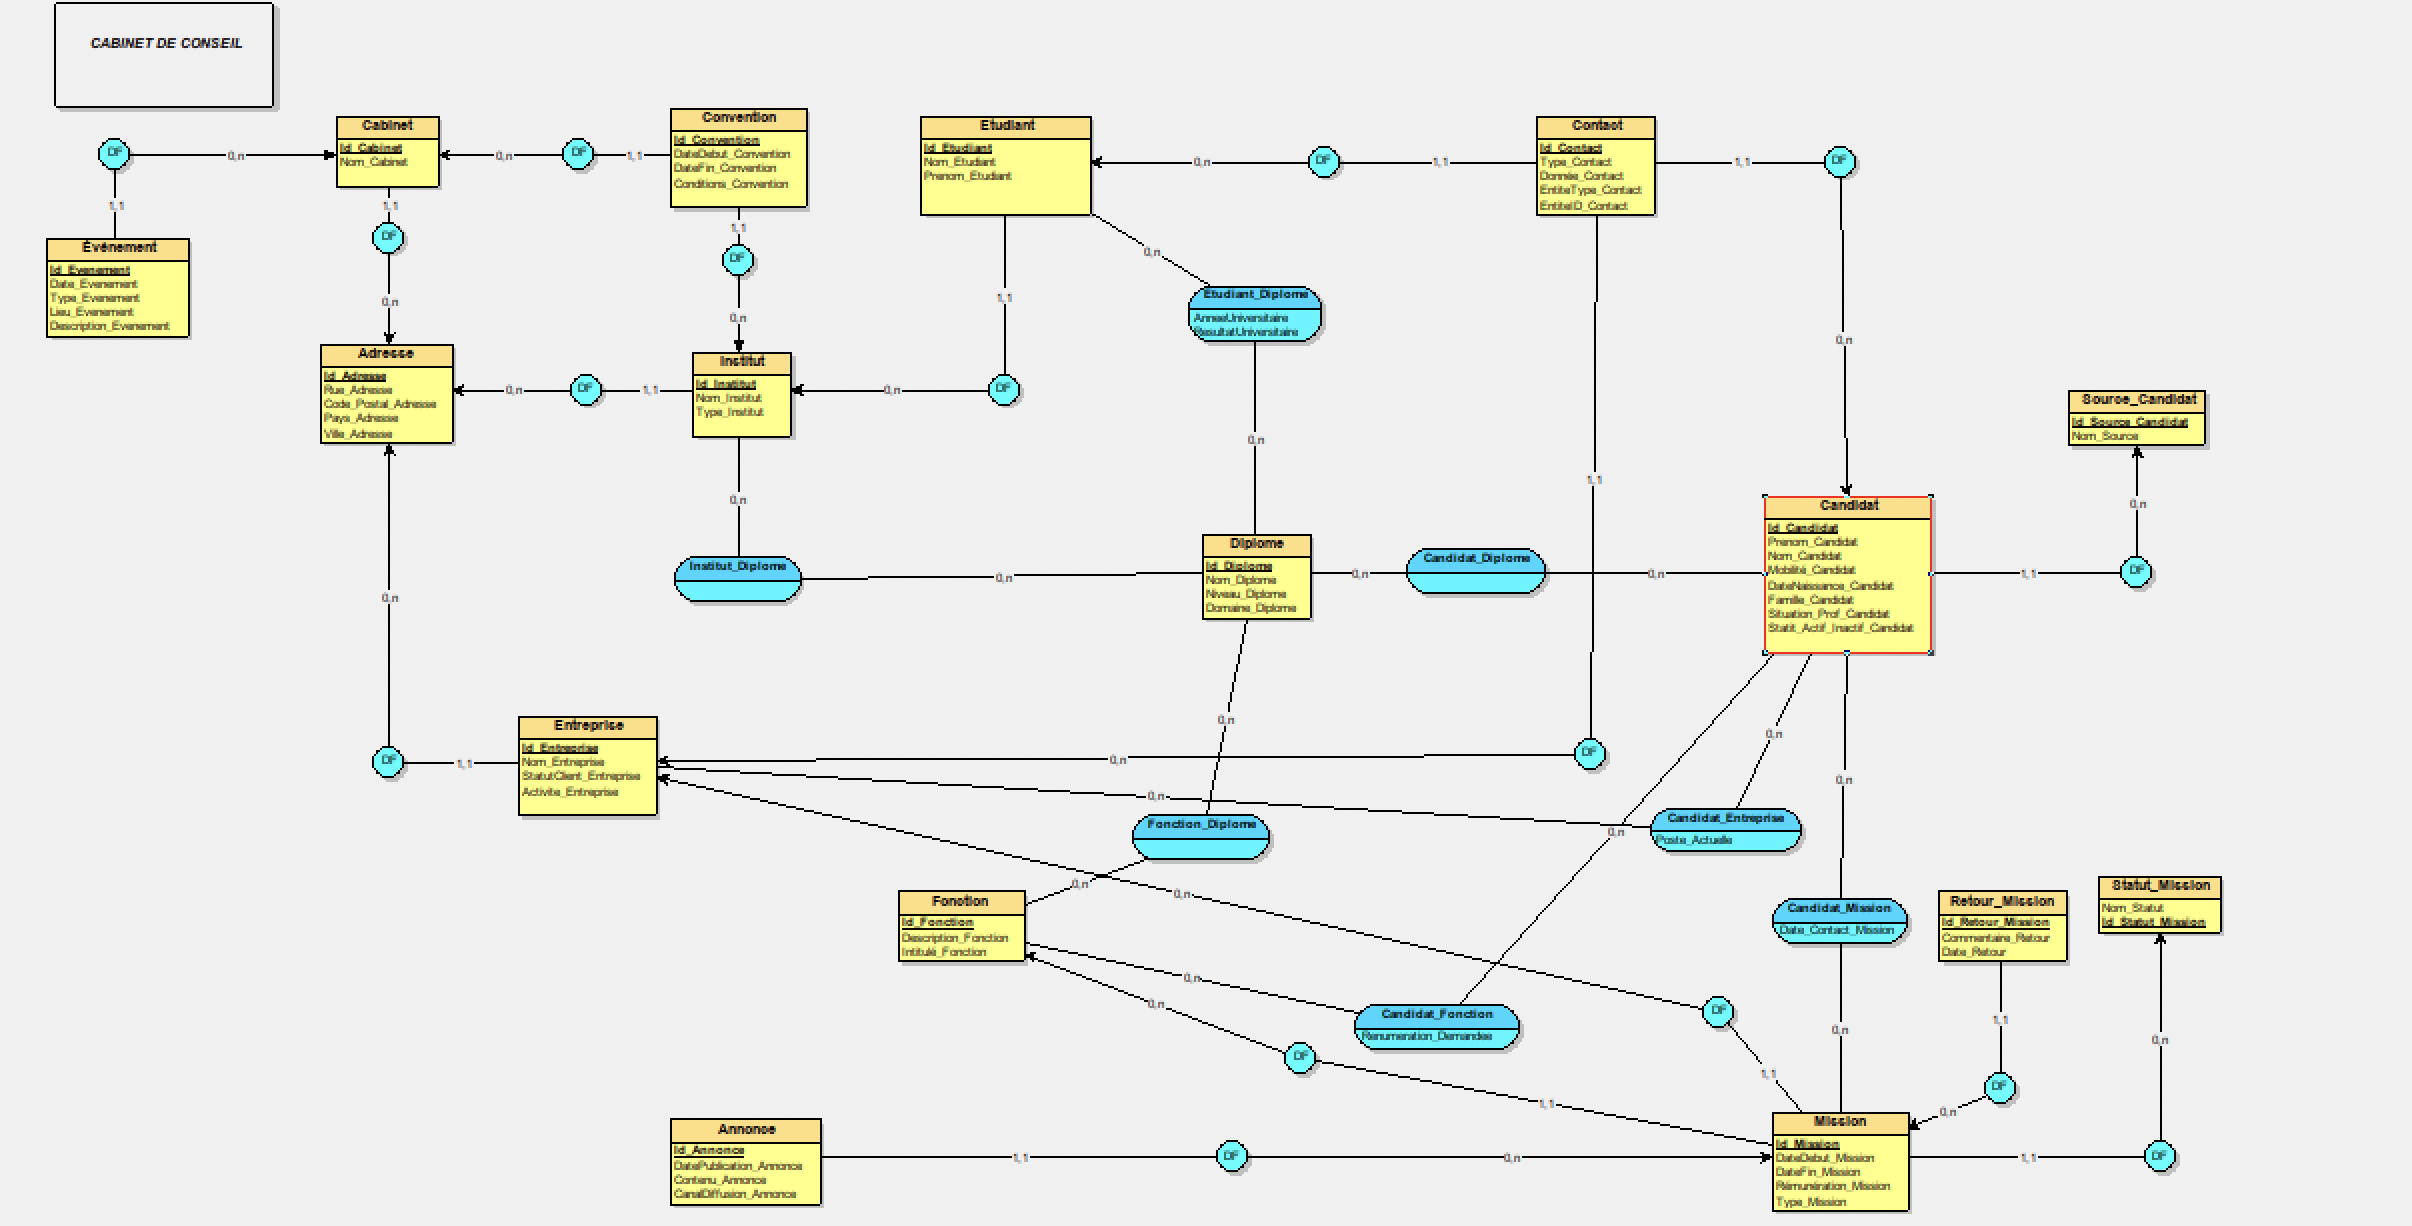
\includegraphics[width=0.8\textwidth]{MCD.png} 
    \caption{Modèle Conceptuel de Données (MCD)}
    \label{fig:mcd}
\end{figure}

\noindent
Les entités principales dans ce modèle sont :
\begin{itemize}
    \item \textbf{Candidat} : Personne postulant pour des missions.
    \item \textbf{Entreprise} : Organisation qui propose des missions.
    \item \textbf{Mission} : Tâche ou projet nécessitant un candidat.
    \item \textbf{Fonction} : Type de poste disponible pour les candidats.
    \item \textbf{Diplôme} : Qualification détenue par un candidat.
    \item \textbf{Institut} : Établissement qui délivre des diplômes.
    \item \textbf{Annonce} : Publication d'une mission.
    \item \textbf{Convention} : Accord entre un institut et un cabinet de conseil.
\end{itemize}

Les relations entre ces entités ont également été définies, telles que les relations \textit{Candidat-Fonction}, \textit{Entreprise-Mission}, et \textit{Candidat-Diplôme}.

\subsection*{2. Modèle Physique de Données (MPD)}

Le \textbf{Modèle Physique de Données} (MPD) est la mise en œuvre concrète du MCD sous forme de tables, de colonnes et de contraintes. Il permet de définir comment les données seront effectivement stockées en base de données.

\begin{figure}[h!]
    \centering
    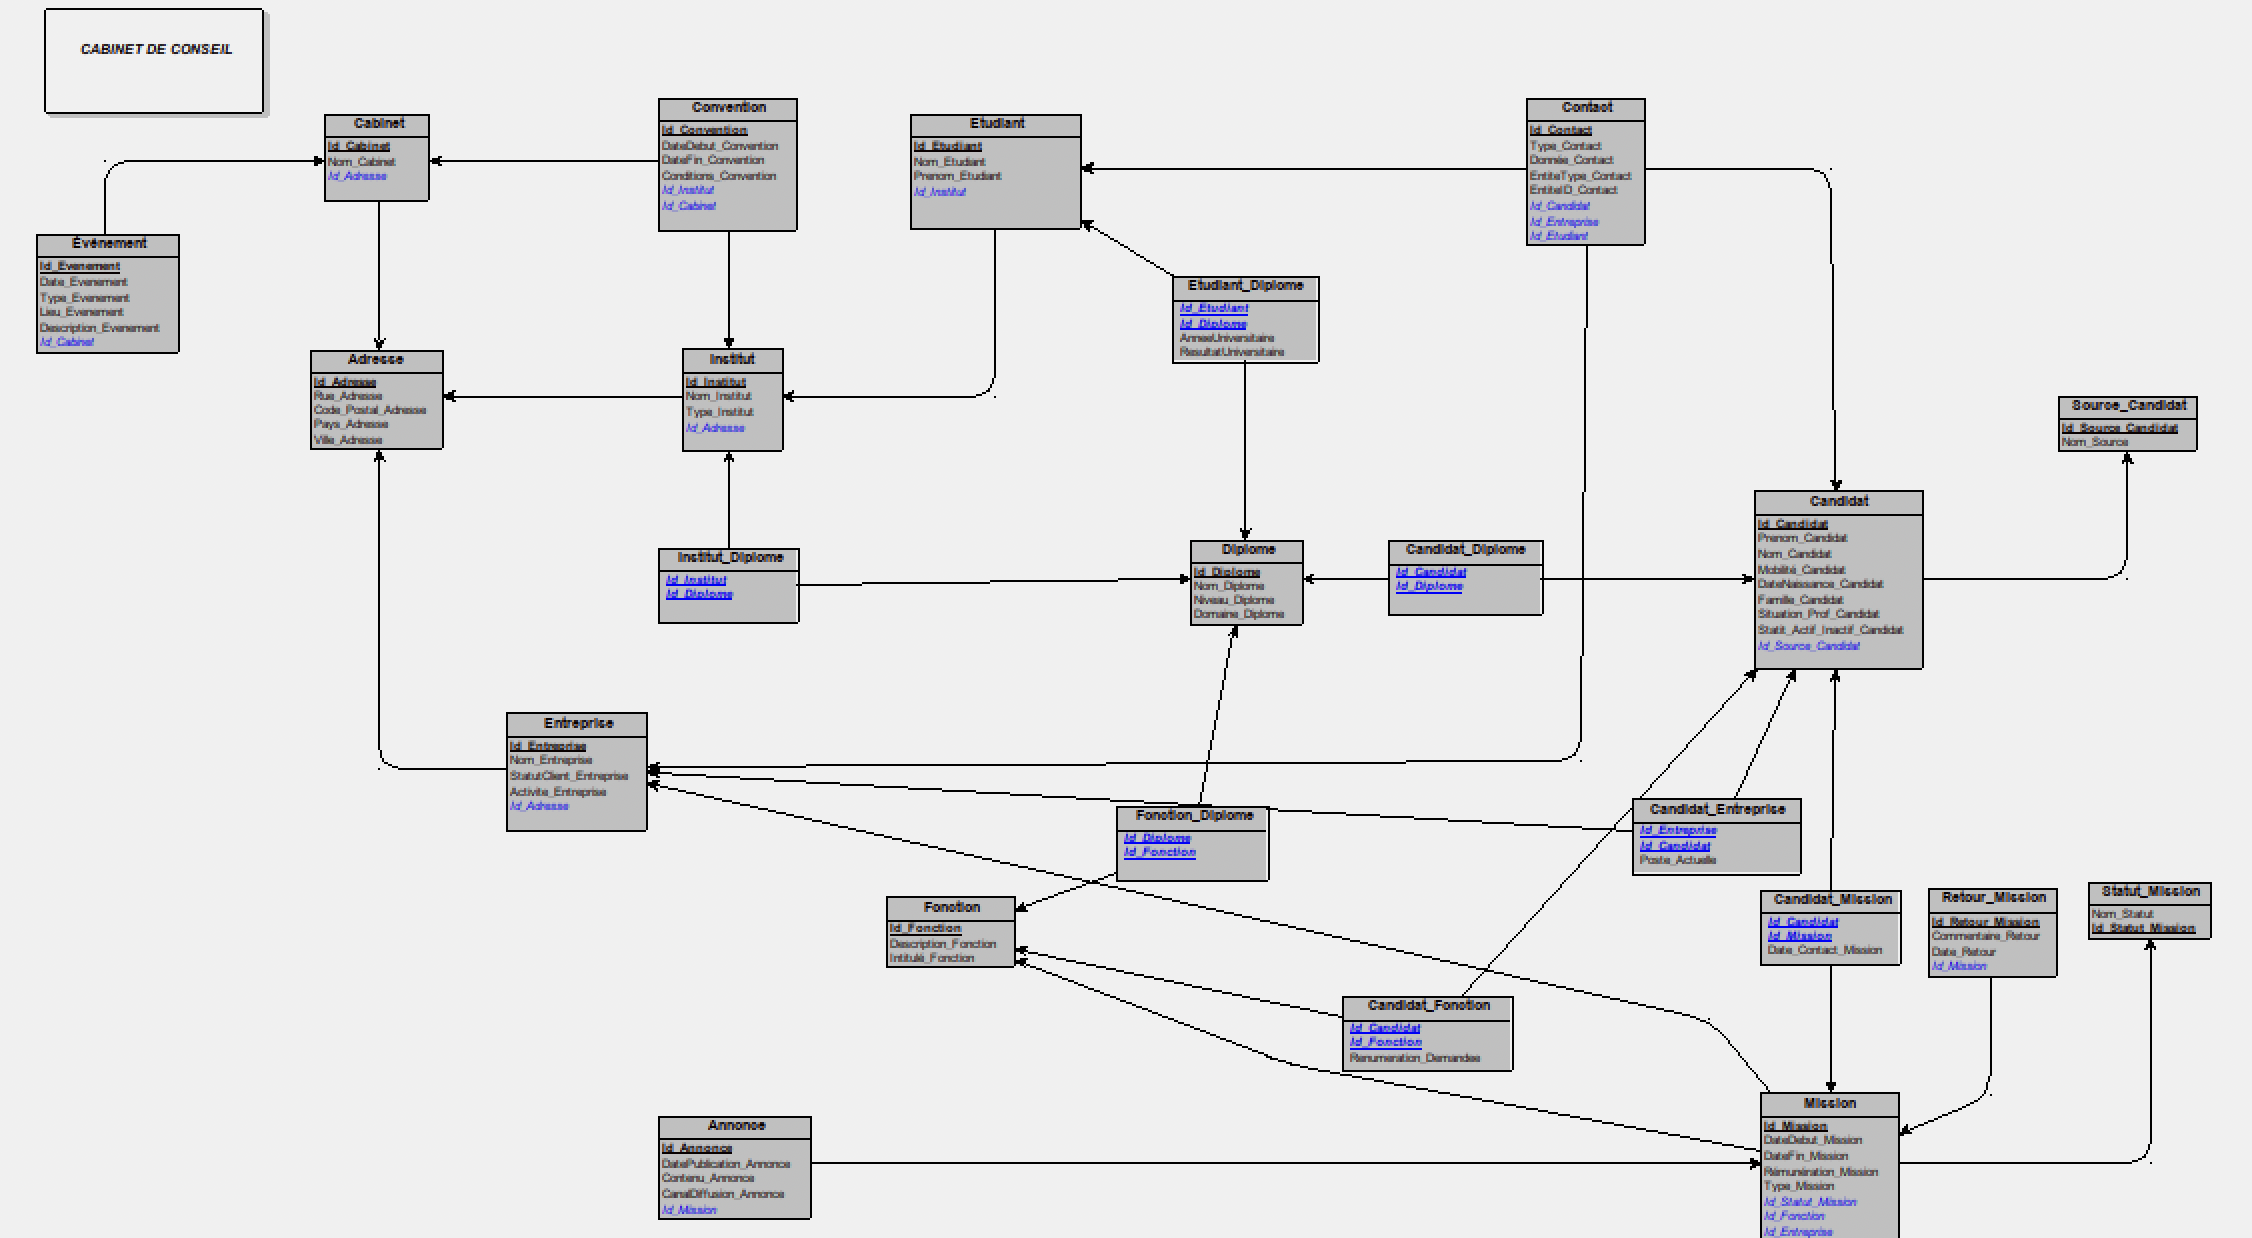
\includegraphics[width=0.8\textwidth]{MPD.png} % Remplacez "MPD.png" par le nom de votre fichier d'image pour le MPD
    \caption{Modèle Physique de Données (MPD)}
    \label{fig:mpd}
\end{figure}

\noindent
Le MPD définit les tables suivantes avec leurs attributs :
\begin{itemize}
    \item \textbf{Candidat} : contient des informations sur les candidats.
    \item \textbf{Entreprise} : informations sur les entreprises.
    \item \textbf{Mission} : les missions proposées par les entreprises.
    \item \textbf{Fonction} : les différents types de fonctions dans les missions.
    \item \textbf{Diplôme} : les diplômes obtenus par les candidats.
    \item \textbf{Institut} : les instituts où les diplômes sont délivrés.
    \item \textbf{Convention} : les conventions entre les instituts et les cabinets.
\end{itemize}

Les tables sont reliées entre elles par des clés étrangères qui permettent de maintenir l'intégrité référentielle.

\subsection*{3. Modèle Logique de Données (MLD)}

Le \textbf{Modèle Logique de Données} (MLD) représente la version logique du modèle de données adapté à une base de données relationnelle. Voici la structure détaillée des tables pour la version Looping (certaines différences par rapport à Oracle) :

\begin{itemize}
    \item \textbf{Diplome} = (\texttt{Id\_Diplome COUNTER}, \texttt{Nom\_Diplome VARCHAR(50)}, \texttt{Niveau\_Diplome VARCHAR(50)}, \texttt{Domaine\_Diplome VARCHAR(50)})
    \item \textbf{Fonction} = (\texttt{Id\_Fonction COUNTER}, \texttt{Description\_Fonction VARCHAR(50)}, \texttt{Intitulé\_Fonction VARCHAR(50)})
    \item \textbf{Source\_Candidat} = (\texttt{Id\_Source\_Candidat COUNTER}, \texttt{Nom\_Source VARCHAR(50)})
    \item \textbf{Statut\_Mission} = (\texttt{Id\_Statut\_Mission COUNTER}, \texttt{Nom\_Statut VARCHAR(50)})
    \item \textbf{Adresse} = (\texttt{Id\_Adresse COUNTER}, \texttt{Rue\_Adresse VARCHAR(100)}, \texttt{Code\_Postal\_Adresse VARCHAR(50)}, \texttt{Pays\_Adresse VARCHAR(100)}, \texttt{Ville\_Adresse VARCHAR(100)})
    \item \textbf{Entreprise} = (\texttt{Id\_Entreprise COUNTER}, \texttt{Nom\_Entreprise VARCHAR(50)}, \texttt{StatutClient\_Entreprise LOGICAL}, \texttt{Activite\_Entreprise VARCHAR(50)}, \texttt{\#Id\_Adresse})
    \item \textbf{Candidat} = (\texttt{Id\_Candidat COUNTER}, \texttt{Prenom\_Candidat VARCHAR(50)}, \texttt{Nom\_Candidat VARCHAR(50)}, \texttt{Mobilite\_Candidat LOGICAL}, \texttt{DateNaissance\_Candidat DATE}, \texttt{Famille\_Candidat VARCHAR(50)}, \texttt{Situation\_Prof\_Candidat VARCHAR(50)}, \texttt{Statut\_Actif\_Inactif\_Candidat LOGICAL}, \texttt{\#Id\_Source\_Candidat})
    \item \textbf{Institut} = (\texttt{Id\_Institut COUNTER}, \texttt{Nom\_Institut VARCHAR(50)}, \texttt{Type\_Institut VARCHAR(50)}, \texttt{\#Id\_Adresse})
    \item \textbf{Mission} = (\texttt{Id\_Mission COUNTER}, \texttt{DateDebut\_Mission DATE}, \texttt{DateFin\_Mission DATE}, \texttt{Rémunération\_Mission CURRENCY}, \texttt{Type\_Mission VARCHAR(50)}, \texttt{\#Id\_Statut\_Mission}, \texttt{\#Id\_Fonction}, \texttt{\#Id\_Entreprise})
    \item \textbf{Cabinet} = (\texttt{Id\_Cabinet COUNTER}, \texttt{Nom\_Cabinet VARCHAR(50)}, \texttt{\#Id\_Adresse})
\end{itemize}

\noindent
Cette version est adaptée pour un environnement Looping, où certaines spécifications diffèrent d'Oracle, notamment en ce qui concerne les \texttt{COUNTER} remplacés par des \texttt{NUMBER} pour l'ID.

\subsection*{4. Analyse des Dépendances Fonctionnelles}

Les dépendances fonctionnelles sont des relations qui définissent comment une donnée peut être déterminée à partir d'autres données. Cela garantit que la base de données soit cohérente et normalisée.

\subsubsection*{Exemples de Dépendances Fonctionnelles}

\begin{itemize}
    \item \textbf{Candidat} : 
    \begin{equation*}
        \text{Id\_Candidat} \rightarrow \text{Prenom\_Candidat}, \text{Nom\_Candidat}, \text{Mobilite\_Candidat}, \text{DateNaissance\_Candidat}, \text{Famille\_Candidat}, \text{Situation\_Prof\_Candidat}, \text{Id\_Source\_Candidat}
    \end{equation*}
    La clé primaire \texttt{Id\_Candidat} détermine de manière unique toutes les informations d'un candidat.
    
    \item \textbf{Candidat\_Fonction} : 
    \begin{equation*}
        \text{Id\_Candidat, Id\_Fonction} \rightarrow \text{Remuneration\_Demandee}
    \end{equation*}
    L'association unique entre un candidat et une fonction détermine la rémunération demandée.
    
    \item \textbf{Mission} : 
    \begin{equation*}
        \text{Id\_Mission} \rightarrow \text{DateDebut\_Mission}, \text{DateFin\_Mission}, \text{Remuneration\_Mission}, \text{Type\_Mission}, \text{Id\_Statut\_Mission}, \text{Id\_Fonction}, \text{Id\_Entreprise}
    \end{equation*}
    La clé primaire \texttt{Id\_Mission} détermine toutes les informations relatives à une mission spécifique.
\end{itemize}

\noindent
Les clés choisies pour assurer l'intégrité et l'unicité des données dans chaque table sont :
\begin{itemize}
    \item \textbf{Candidat} : \texttt{Id\_Candidat}
    \item \textbf{Entreprise} : \texttt{Id\_Entreprise}
    \item \textbf{Mission} : \texttt{Id\_Mission}
    \item \textbf{Fonction} : \texttt{Id\_Fonction}
    \item \textbf{Diplôme} : \texttt{Id\_Diplome}
    \item \textbf{Institut} : \texttt{Id\_Institut}
    \item \textbf{Convention} : \texttt{Id\_Convention}
    \item \textbf{Candidat\_Fonction} : \texttt{Id\_Candidat, Id\_Fonction}
    \item \textbf{Candidat\_Diplome} : \texttt{Id\_Candidat, Id\_Diplome}
\end{itemize}

Ces clés permettent de garantir que chaque enregistrement est unique et d'assurer une bonne gestion des relations entre les tables, facilitant ainsi la gestion et la recherche des données.


\subsection*{5. Création de la Base de Données}

La base de données a été créée en utilisant les modèles MCD et MPD. Les tables ont été créées en respectant les dépendances fonctionnelles et les clés primaires définies. Les données peuvent maintenant être insérées et gérées à l'aide de requêtes SQL.

\subsubsection*{Séquences }
Lors de l’ajout de nouvelles lignes dans une table, les séquences peuvent être utilisées pour générer automatiquement des valeurs uniques pour les clés primaires sans avoir à les gérer manuellement.
Et le cache  de 100 valeurs de la séquence à l’avance est pour améliorer les performances en cas de demandes multiples


\subsubsection*{Code Sql de la Création de la Base de Données}





\begin{verbatim}
    -- Sequences
    CREATE SEQUENCE seq_diplome START WITH 1 INCREMENT BY 1 CACHE 100;
    CREATE SEQUENCE seq_fonction START WITH 1 INCREMENT BY 1 CACHE 100;
    CREATE SEQUENCE seq_source_candidat START WITH 1 INCREMENT BY 1 CACHE 100;
    CREATE SEQUENCE seq_statut_mission START WITH 1 INCREMENT BY 1 CACHE 100;
    CREATE SEQUENCE seq_adresse START WITH 1 INCREMENT BY 1 CACHE 100;
    CREATE SEQUENCE seq_entreprise START WITH 1 INCREMENT BY 1 CACHE 100;
    CREATE SEQUENCE seq_candidat START WITH 1 INCREMENT BY 1 CACHE 100;
    CREATE SEQUENCE seq_institut START WITH 1 INCREMENT BY 1 CACHE 100; 
    CREATE SEQUENCE seq_mission START WITH 1 INCREMENT BY 1 CACHE 100;
    CREATE SEQUENCE seq_cabinet START WITH 1 INCREMENT BY 1 CACHE 100;
    CREATE SEQUENCE seq_convention START WITH 1 INCREMENT BY 1 CACHE 100;
    CREATE SEQUENCE seq_annonce START WITH 1 INCREMENT BY 1 CACHE 100;
    CREATE SEQUENCE seq_evenement START WITH 1 INCREMENT BY 1 CACHE 100;
    CREATE SEQUENCE seq_retour_mission START WITH 1 INCREMENT BY 1 CACHE 100;
    CREATE SEQUENCE seq_etudiant START WITH 1 INCREMENT BY 1 CACHE 100;
    CREATE SEQUENCE seq_contact START WITH 1 INCREMENT BY 1 CACHE 100; 
    
    -- Tables
    CREATE TABLE Diplome(
       Id_Diplome NUMBER PRIMARY KEY,
       Nom_Diplome VARCHAR2(50),
       Niveau_Diplome VARCHAR2(50),
       Domaine_Diplome VARCHAR2(50)
    );
    
    CREATE TABLE Fonction(
       Id_Fonction NUMBER PRIMARY KEY,
       Description_Fonction VARCHAR2(50),
       Intitule_Fonction VARCHAR2(50)
    );
    
    CREATE TABLE Source_Candidat(
       Id_Source_Candidat NUMBER PRIMARY KEY,
       Nom_Source VARCHAR2(50)
    );
    
    CREATE TABLE Statut_Mission(
       Id_Statut_Mission NUMBER PRIMARY KEY,
       Nom_Statut VARCHAR2(50)
    );
    
    CREATE TABLE Adresse(
       Id_Adresse NUMBER PRIMARY KEY,
       Rue_Adresse VARCHAR2(100),
       Code_Postal_Adresse VARCHAR2(50),
       Pays_Adresse VARCHAR2(100),
       Ville_Adresse VARCHAR2(100)
    );
    
    CREATE TABLE Entreprise(
       Id_Entreprise NUMBER PRIMARY KEY,
       Nom_Entreprise VARCHAR2(50),
       StatutClient_Entreprise NUMBER(1),  -- 1 pour TRUE, 0 pour FALSE
       Activite_Entreprise VARCHAR2(50),
       Id_Adresse NUMBER NOT NULL,
       FOREIGN KEY(Id_Adresse) REFERENCES Adresse(Id_Adresse)
    );
    
    CREATE TABLE Candidat(
       Id_Candidat NUMBER PRIMARY KEY,
       Prenom_Candidat VARCHAR2(50),
       Nom_Candidat VARCHAR2(50),
       Mobilite_Candidat NUMBER(1),  -- 1 pour TRUE, 0 pour FALSE
       Statut_Actif_Inactif_Candidat NUMBER(1) DEFAULT 1,  -- 1 pour TRUE, 0 pour FALSE 
       DateNaissance_Candidat DATE,
       Famille_Candidat VARCHAR2(50),
       Situation_Prof_Candidat VARCHAR2(50),
       Id_Source_Candidat NUMBER NOT NULL,
       FOREIGN KEY(Id_Source_Candidat) REFERENCES Source_Candidat(Id_Source_Candidat)
    );
    
    CREATE TABLE Institut(
       Id_Institut NUMBER PRIMARY KEY,
       Nom_Institut VARCHAR2(50),
       Type_Institut VARCHAR2(50),
       Id_Adresse NUMBER NOT NULL,
       FOREIGN KEY(Id_Adresse) REFERENCES Adresse(Id_Adresse)
    );
    
    CREATE TABLE Mission(
       Id_Mission NUMBER PRIMARY KEY,
       DateDebut_Mission DATE,
       DateFin_Mission DATE,
       Remuneration_Mission NUMBER(15,2),
       Type_Mission VARCHAR2(50),
       Id_Statut_Mission NUMBER NOT NULL,
       Id_Fonction NUMBER NOT NULL,
       Id_Entreprise NUMBER NOT NULL,
       FOREIGN KEY(Id_Statut_Mission) REFERENCES Statut_Mission(Id_Statut_Mission),
       FOREIGN KEY(Id_Fonction) REFERENCES Fonction(Id_Fonction),
       FOREIGN KEY(Id_Entreprise) REFERENCES Entreprise(Id_Entreprise)
    );
    
    CREATE TABLE Cabinet(
       Id_Cabinet NUMBER PRIMARY KEY,
       Nom_Cabinet VARCHAR2(50),
       Id_Adresse NUMBER NOT NULL,
       FOREIGN KEY(Id_Adresse) REFERENCES Adresse(Id_Adresse)
    );
    
    CREATE TABLE Convention(
       Id_Convention NUMBER PRIMARY KEY,
       DateDebut_Convention DATE,
       DateFin_Convention DATE,
       Conditions_Convention VARCHAR2(255),
       Id_Institut NUMBER NOT NULL,
       Id_Cabinet NUMBER NOT NULL,
       FOREIGN KEY(Id_Institut) REFERENCES Institut(Id_Institut) ON DELETE CASCADE,
       FOREIGN KEY(Id_Cabinet) REFERENCES Cabinet(Id_Cabinet) ON DELETE CASCADE
    );
    
    CREATE TABLE Annonce(
       Id_Annonce NUMBER PRIMARY KEY,
       DatePublication_Annonce DATE,
       Contenu_Annonce CLOB,
       CanalDiffusion_Annonce VARCHAR2(50),
       Id_Mission NUMBER NOT NULL,
       FOREIGN KEY(Id_Mission) REFERENCES Mission(Id_Mission) ON DELETE CASCADE
    );
    
    CREATE TABLE Evenement(
       Id_Evenement NUMBER PRIMARY KEY,
       Date_Evenement DATE,
       Type_Evenement VARCHAR2(50),
       Lieu_Evenement VARCHAR2(50),
       Description_Evenement VARCHAR2(50),
       Id_Cabinet NUMBER NOT NULL,
       FOREIGN KEY(Id_Cabinet) REFERENCES Cabinet(Id_Cabinet) ON DELETE CASCADE
    );
    
    CREATE TABLE Retour_Mission(
       Id_Retour_Mission NUMBER PRIMARY KEY,
       Commentaire_Retour CLOB,
       Date_Retour DATE,
       Id_Mission NUMBER NOT NULL,
       FOREIGN KEY(Id_Mission) REFERENCES Mission(Id_Mission) ON DELETE CASCADE
    );
    
    CREATE TABLE Etudiant(
       Id_Etudiant NUMBER PRIMARY KEY,
       Nom_Etudiant VARCHAR2(50),
       Prenom_Etudiant VARCHAR2(50),
       Id_Institut NUMBER NOT NULL,
       FOREIGN KEY(Id_Institut) REFERENCES Institut(Id_Institut)
    );
    
    CREATE TABLE Contact(
       Id_Contact NUMBER PRIMARY KEY,
       Type_Contact VARCHAR2(50) NOT NULL,
       Donnee_Contact VARCHAR2(50) NOT NULL,
       EntiteType_Contact VARCHAR2(50),
       EntiteID_Contact NUMBER,
       Id_Candidat NUMBER,
       Id_Entreprise NUMBER,
       Id_Etudiant NUMBER,
       FOREIGN KEY(Id_Candidat) REFERENCES Candidat(Id_Candidat) ON DELETE CASCADE,
       FOREIGN KEY(Id_Entreprise) REFERENCES Entreprise(Id_Entreprise) ON DELETE CASCADE,
       FOREIGN KEY(Id_Etudiant) REFERENCES Etudiant(Id_Etudiant) ON DELETE CASCADE,
       CHECK (
         (Id_Candidat IS NOT NULL AND Id_Entreprise IS NULL AND Id_Etudiant IS NULL) OR
         (Id_Candidat IS NULL AND Id_Entreprise IS NOT NULL AND Id_Etudiant IS NULL) OR
         (Id_Candidat IS NULL AND Id_Entreprise IS NULL AND Id_Etudiant IS NOT NULL)
       )
    );
    
    CREATE TABLE Candidat_Diplome(
       Id_Candidat NUMBER,
       Id_Diplome NUMBER,
       PRIMARY KEY(Id_Candidat, Id_Diplome),
       FOREIGN KEY(Id_Candidat) REFERENCES Candidat(Id_Candidat) ON DELETE CASCADE,
       FOREIGN KEY(Id_Diplome) REFERENCES Diplome(Id_Diplome) ON DELETE CASCADE
    );
    
    CREATE TABLE Fonction_Diplome(
       Id_Diplome NUMBER,
       Id_Fonction NUMBER,
       PRIMARY KEY(Id_Diplome, Id_Fonction),
       FOREIGN KEY(Id_Diplome) REFERENCES Diplome(Id_Diplome) ON DELETE CASCADE,
       FOREIGN KEY(Id_Fonction) REFERENCES Fonction(Id_Fonction) ON DELETE CASCADE
    );
    
    CREATE TABLE Candidat_Fonction(
       Id_Candidat NUMBER,
       Id_Fonction NUMBER,
       Remuneration_Demandee NUMBER(10,2),
       PRIMARY KEY(Id_Candidat, Id_Fonction),
       FOREIGN KEY(Id_Candidat) REFERENCES Candidat(Id_Candidat) ON DELETE CASCADE,
       FOREIGN KEY(Id_Fonction) REFERENCES Fonction(Id_Fonction) ON DELETE CASCADE
    );
    
    CREATE TABLE Candidat_Mission(
       Id_Candidat NUMBER,
       Id_Mission NUMBER,
       Date_Contact_Mission DATE,
       PRIMARY KEY(Id_Candidat, Id_Mission),
       FOREIGN KEY(Id_Candidat) REFERENCES Candidat(Id_Candidat) ON DELETE CASCADE,
       FOREIGN KEY(Id_Mission) REFERENCES Mission(Id_Mission) ON DELETE CASCADE
    );
    
    CREATE TABLE Institut_Diplome(
       Id_Institut NUMBER,
       Id_Diplome NUMBER,
       PRIMARY KEY(Id_Institut, Id_Diplome),
       FOREIGN KEY(Id_Institut) REFERENCES Institut(Id_Institut) ON DELETE CASCADE,
       FOREIGN KEY(Id_Diplome) REFERENCES Diplome(Id_Diplome) ON DELETE CASCADE
    );
    
    CREATE TABLE Etudiant_Diplome(
       Id_Etudiant NUMBER,
       Id_Diplome NUMBER,
       AnneeUniversitaire VARCHAR2(10),
       ResultatUniversitaire VARCHAR2(255),
       PRIMARY KEY(Id_Etudiant, Id_Diplome),
       FOREIGN KEY(Id_Etudiant) REFERENCES Etudiant(Id_Etudiant) ON DELETE CASCADE,
       FOREIGN KEY(Id_Diplome) REFERENCES Diplome(Id_Diplome) ON DELETE CASCADE
    );
    
    CREATE TABLE Candidat_Entreprise(
       Id_Entreprise NUMBER,
       Id_Candidat NUMBER,
       Poste_Actuelle VARCHAR2(50),
       PRIMARY KEY(Id_Entreprise, Id_Candidat),
       FOREIGN KEY(Id_Entreprise) REFERENCES Entreprise(Id_Entreprise) ON DELETE CASCADE,
       FOREIGN KEY(Id_Candidat) REFERENCES Candidat(Id_Candidat) ON DELETE CASCADE
    );
    
\end{verbatim}
\subsection*{5. Triggers avant insertion}

Les triggers vérifient si la valeur d’un identifiant spécifique (Id_*) est fournie lors de l’insertion d’une nouvelle ligne dans la table.
\subsubsection*{Code Sql des Triggers avant insertion}

\begin{verbatim}
CREATE OR REPLACE TRIGGER trg_diplome_avant_insertion
BEFORE INSERT ON Diplome
FOR EACH ROW
BEGIN
   IF :NEW.Id_Diplome IS NULL THEN
      SELECT seq_diplome.NEXTVAL INTO :NEW.Id_Diplome FROM dual;
   END IF;
END;
/

CREATE OR REPLACE TRIGGER trg_fonction_avant_insertion
BEFORE INSERT ON Fonction
FOR EACH ROW
BEGIN
   IF :NEW.Id_Fonction IS NULL THEN
      SELECT seq_fonction.NEXTVAL INTO :NEW.Id_Fonction FROM dual;
   END IF;
END;
/


CREATE OR REPLACE TRIGGER trg_source_candidat_avant_insertion
BEFORE INSERT ON Source_Candidat
FOR EACH ROW
BEGIN
   IF :NEW.Id_Source_Candidat IS NULL THEN
      SELECT seq_source_candidat.NEXTVAL INTO :NEW.Id_Source_Candidat FROM dual;
   END IF;
END;
/

CREATE OR REPLACE TRIGGER trg_statut_mission_avant_insertion
BEFORE INSERT ON Statut_Mission
FOR EACH ROW
BEGIN
   IF :NEW.Id_Statut_Mission IS NULL THEN
      SELECT seq_statut_mission.NEXTVAL INTO :NEW.Id_Statut_Mission FROM dual;
   END IF;
END;
/

CREATE OR REPLACE TRIGGER trg_adresse_avant_insertion
BEFORE INSERT ON Adresse
FOR EACH ROW
BEGIN
   IF :NEW.Id_Adresse IS NULL THEN
      SELECT seq_adresse.NEXTVAL INTO :NEW.Id_Adresse FROM dual;
   END IF;
END;
/

CREATE OR REPLACE TRIGGER trg_entreprise_avant_insertion
BEFORE INSERT ON Entreprise
FOR EACH ROW
BEGIN
   IF :NEW.Id_Entreprise IS NULL THEN
      SELECT seq_entreprise.NEXTVAL INTO :NEW.Id_Entreprise FROM dual;
   END IF;
END;
/

CREATE OR REPLACE TRIGGER trg_candidat_avant_insertion
BEFORE INSERT ON Candidat
FOR EACH ROW
BEGIN
   IF :NEW.Id_Candidat IS NULL THEN
      SELECT seq_candidat.NEXTVAL INTO :NEW.Id_Candidat FROM dual;
   END IF;
END;
/

CREATE OR REPLACE TRIGGER trg_institut_avant_insertion
BEFORE INSERT ON Institut
FOR EACH ROW
BEGIN
   IF :NEW.Id_Institut IS NULL THEN
      SELECT seq_institut.NEXTVAL INTO :NEW.Id_Institut FROM dual;
   END IF;
END;
/

CREATE OR REPLACE TRIGGER trg_mission_avant_insertion
BEFORE INSERT ON Mission
FOR EACH ROW
BEGIN
   IF :NEW.Id_Mission IS NULL THEN
      SELECT seq_mission.NEXTVAL INTO :NEW.Id_Mission FROM dual;
   END IF;
END;
/

CREATE OR REPLACE TRIGGER trg_cabinet_avant_insertion
BEFORE INSERT ON Cabinet
FOR EACH ROW
BEGIN
   IF :NEW.Id_Cabinet IS NULL THEN
      SELECT seq_cabinet.NEXTVAL INTO :NEW.Id_Cabinet FROM dual;
   END IF;
END;
/

CREATE OR REPLACE TRIGGER trg_convention_avant_insertion
BEFORE INSERT ON Convention
FOR EACH ROW
BEGIN
   IF :NEW.Id_Convention IS NULL THEN
      SELECT seq_convention.NEXTVAL INTO :NEW.Id_Convention FROM dual;
   END IF;
END;
/

CREATE OR REPLACE TRIGGER trg_annonce_avant_insertion
BEFORE INSERT ON Annonce
FOR EACH ROW
BEGIN
   IF :NEW.Id_Annonce IS NULL THEN
      SELECT seq_annonce.NEXTVAL INTO :NEW.Id_Annonce FROM dual;
   END IF;
END;
/

CREATE OR REPLACE TRIGGER trg_evenement_avant_insertion
BEFORE INSERT ON Evenement
FOR EACH ROW
BEGIN
   IF :NEW.Id_Evenement IS NULL THEN
      SELECT seq_evenement.NEXTVAL INTO :NEW.Id_Evenement FROM dual;
   END IF;
END;
/

CREATE OR REPLACE TRIGGER trg_retour_mission_avant_insertion
BEFORE INSERT ON Retour_Mission
FOR EACH ROW
BEGIN
   IF :NEW.Id_Retour_Mission IS NULL THEN
      SELECT seq_retour_mission.NEXTVAL INTO :NEW.Id_Retour_Mission FROM dual;
   END IF;
END;
/

CREATE OR REPLACE TRIGGER trg_etudiant_avant_insertion
BEFORE INSERT ON Etudiant
FOR EACH ROW
BEGIN
   IF :NEW.Id_Etudiant IS NULL THEN
      SELECT seq_etudiant.NEXTVAL INTO :NEW.Id_Etudiant FROM dual;
   END IF;
END;
/

CREATE OR REPLACE TRIGGER trg_candidat_fonction_avant_insertion
BEFORE INSERT ON Candidat_Fonction
FOR EACH ROW
BEGIN
   IF :NEW.Id_Candidat IS NULL THEN
      RAISE_APPLICATION_ERROR(-20001, 'Id_Candidat ne peut pas être NULL');
   END IF;
   IF :NEW.Id_Fonction IS NULL THEN
      RAISE_APPLICATION_ERROR(-20002, 'Id_Fonction ne peut pas être NULL');
   END IF;
   IF :NEW.Remuneration_Demandee IS NULL THEN
      :NEW.Remuneration_Demandee := 0; -- Valeur par défaut si nécessaire
   END IF;
END;
/

CREATE OR REPLACE TRIGGER trg_contact_avant_insertion
BEFORE INSERT ON Contact
FOR EACH ROW
BEGIN
   IF :NEW.Id_Contact IS NULL THEN
      SELECT seq_contact.NEXTVAL INTO :NEW.Id_Contact FROM dual;
   END IF;
END;
/


-- Insertion dans Diplome
INSERT INTO Diplome (Nom_Diplome, Niveau_Diplome, Domaine_Diplome)
VALUES ('Master en Informatique', 'Master', 'Informatique');

INSERT INTO Diplome (Nom_Diplome, Niveau_Diplome, Domaine_Diplome)
VALUES ('Licence en Gestion', 'Licence', 'Gestion');


-- Insertion dans Fonction
INSERT INTO Fonction (Description_Fonction, Intitule_Fonction)
VALUES ('Développement de logiciels', 'Développeur');

INSERT INTO Fonction (Description_Fonction, Intitule_Fonction)
VALUES ('Gestion de projet', 'Chef de Projet');


-- Insertion dans Source_Candidat
INSERT INTO Source_Candidat (Nom_Source)
VALUES ('LinkedIn');

INSERT INTO Source_Candidat (Nom_Source)
VALUES ('Indeed');

-- Insertion dans Statut_Mission
INSERT INTO Statut_Mission (Nom_Statut)
VALUES ('En cours');

INSERT INTO Statut_Mission (Nom_Statut)
VALUES ('Terminée');

-- Insertion dans Adresse
INSERT INTO Adresse (Rue_Adresse, Code_Postal_Adresse, Pays_Adresse, Ville_Adresse)
VALUES ('123 Rue Exemple', '75000', 'France', 'Paris');

INSERT INTO Adresse (Rue_Adresse, Code_Postal_Adresse, Pays_Adresse, Ville_Adresse)
VALUES ('456 Avenue Secondaire', '69000', 'France', 'Lyon');

-- Insertion dans Entreprise
INSERT INTO Entreprise (Nom_Entreprise, StatutClient_Entreprise, Activite_Entreprise, Id_Adresse)
VALUES ('TechCorp', 1, 'Technologie', 1);

INSERT INTO Entreprise (Nom_Entreprise, StatutClient_Entreprise, Activite_Entreprise, Id_Adresse)
VALUES ('FinancePlus', 0, 'Finance', 2);

-- Insertion dans Candidat
INSERT INTO Candidat (Prenom_Candidat, Nom_Candidat, Mobilite_Candidat, DateNaissance_Candidat, Famille_Candidat, Situation_Prof_Candidat, Id_Source_Candidat)
VALUES ('Jean', 'Dupont', 1, TO_DATE('1990-01-01', 'YYYY-MM-DD'), 'Célibataire', 'Actif', 1);

INSERT INTO Candidat (Prenom_Candidat, Nom_Candidat, Mobilite_Candidat, DateNaissance_Candidat, Famille_Candidat, Situation_Prof_Candidat, Id_Source_Candidat)
VALUES ('Marie', 'Curie', 0, TO_DATE('1985-05-15', 'YYYY-MM-DD'), 'Mariée', 'Inactif', 2);


-- Insertion dans Institut
INSERT INTO Institut (Nom_Institut, Type_Institut, Id_Adresse)
VALUES ('Université de Paris', 'Universitaire', 1);

INSERT INTO Institut (Nom_Institut, Type_Institut, Id_Adresse)
VALUES ('Institut Supérieur Lyon', 'Universitaire', 2);

-- Insertion dans Mission
INSERT INTO Mission (DateDebut_Mission, DateFin_Mission, Remuneration_Mission, Type_Mission, Id_Statut_Mission, Id_Fonction, Id_Entreprise)
VALUES (
    TO_DATE('2024-05-01', 'YYYY-MM-DD'), 
    TO_DATE('2024-12-31', 'YYYY-MM-DD'), 
    50000.00, 
    'Développement', 
    1, 
    1, 
    1
);

INSERT INTO Mission (DateDebut_Mission, DateFin_Mission, Remuneration_Mission, Type_Mission, Id_Statut_Mission, Id_Fonction, Id_Entreprise)
VALUES (
    TO_DATE('2024-06-01', 'YYYY-MM-DD'), 
    TO_DATE('2024-11-30', 'YYYY-MM-DD'), 
    40000.00, 
    'Gestion de Projet', 
    2, 
    2, 
    2
);


-- Insertion dans Cabinet
INSERT INTO Cabinet (Nom_Cabinet, Id_Adresse)
VALUES ('Cabinet Consulting', 1);

INSERT INTO Cabinet (Nom_Cabinet, Id_Adresse)
VALUES ('Cabinet Finance', 2);

-- Insertion dans Convention
INSERT INTO Convention (DateDebut_Convention, DateFin_Convention, Conditions_Convention, Id_Institut, Id_Cabinet)
VALUES (
    TO_DATE('2024-01-01', 'YYYY-MM-DD'), 
    TO_DATE('2024-12-31', 'YYYY-MM-DD'), 
    'Conditions standards', 
    1, 
    1
);

INSERT INTO Convention (DateDebut_Convention, DateFin_Convention, Conditions_Convention, Id_Institut, Id_Cabinet)
VALUES (
    TO_DATE('2024-02-01', 'YYYY-MM-DD'), 
    TO_DATE('2024-11-30', 'YYYY-MM-DD'), 
    'Conditions spécifiques', 
    2, 
    2
);
-- Insertion dans Annonce
INSERT INTO Annonce (DatePublication_Annonce, Contenu_Annonce, CanalDiffusion_Annonce, Id_Mission)
VALUES (
    TO_DATE('2024-04-01', 'YYYY-MM-DD'), 
    'Nous recherchons un développeur expérimenté.', 
    'LinkedIn', 
    1
);

INSERT INTO Annonce (DatePublication_Annonce, Contenu_Annonce, CanalDiffusion_Annonce, Id_Mission)
VALUES (
    TO_DATE('2024-04-15', 'YYYY-MM-DD'), 
    'Chef de projet recherché avec 5 ans d expérience.',
    'Indeed', 
    2
);


-- Insertion dans Evenement
INSERT INTO Evenement (Date_Evenement, Type_Evenement, Lieu_Evenement, Description_Evenement, Id_Cabinet)
VALUES (
    TO_DATE('2024-07-01', 'YYYY-MM-DD'), 
    'Conférence', 
    'Paris', 
    'Conférence sur les nouvelles technologies.', 
    1
);

INSERT INTO Evenement (Date_Evenement, Type_Evenement, Lieu_Evenement, Description_Evenement, Id_Cabinet)
VALUES (
    TO_DATE('2024-08-15', 'YYYY-MM-DD'), 
    'Atelier', 
    'Lyon', 
    'Atelier de gestion de projet.', 
    2
);


-- Insertion dans Retour_Mission
INSERT INTO Retour_Mission (Commentaire_Retour, Date_Retour, Id_Mission)
VALUES (
    'Mission terminée avec succès.',
    TO_DATE('2024-12-31', 'YYYY-MM-DD'),
    1
);

INSERT INTO Retour_Mission (Commentaire_Retour, Date_Retour, Id_Mission)
VALUES (
    'Problèmes rencontrés lors de la gestion des ressources.',
    TO_DATE('2024-11-30', 'YYYY-MM-DD'),
    2
);




-- Insertion dans Etudiant
INSERT INTO Etudiant (Nom_Etudiant, Prenom_Etudiant, Id_Institut)
VALUES ('Martin', 'Lefevre', 1);

INSERT INTO Etudiant (Nom_Etudiant, Prenom_Etudiant, Id_Institut)
VALUES ('Sophie', 'Durand', 2);


-- Insertion dans Contact
INSERT INTO Contact (Type_Contact, Donnee_Contact, EntiteType_Contact, EntiteID_Contact, Id_Candidat, Id_Entreprise, Id_Etudiant)
VALUES ('Email', 'jean.dupont@example.com', 'Candidat', 1, 1, NULL, NULL);

INSERT INTO Contact (Type_Contact, Donnee_Contact, EntiteType_Contact, EntiteID_Contact, Id_Candidat, Id_Entreprise, Id_Etudiant)
VALUES ('Téléphone', '0123456789', 'Entreprise', 2, NULL, 1, NULL);


-- Insertion dans Candidat_Diplome
INSERT INTO Candidat_Diplome (Id_Candidat, Id_Diplome)
VALUES (1, 1);

INSERT INTO Candidat_Diplome (Id_Candidat, Id_Diplome)
VALUES (2, 2);


-- Insertion dans Fonction_Diplome
INSERT INTO Fonction_Diplome (Id_Diplome, Id_Fonction)
VALUES (1, 1);

INSERT INTO Fonction_Diplome (Id_Diplome, Id_Fonction)
VALUES (2, 2);

-- Insertion dans Candidat_Fonction
INSERT INTO Candidat_Fonction (Id_Candidat, Id_Fonction, Remuneration_Demandee)
VALUES (1, 1, 45000.00);

INSERT INTO Candidat_Fonction (Id_Candidat, Id_Fonction, Remuneration_Demandee)
VALUES (2, 2, 50000.00);

-- Insertion dans Candidat_Mission
INSERT INTO Candidat_Mission (Id_Candidat, Id_Mission, Date_Contact_Mission)
VALUES (1, 1, TO_DATE('2024-04-01', 'YYYY-MM-DD'));

INSERT INTO Candidat_Mission (Id_Candidat, Id_Mission, Date_Contact_Mission)
VALUES (2, 2, TO_DATE('2024-05-15', 'YYYY-MM-DD'));

-- Insertion dans Institut_Diplome
INSERT INTO Institut_Diplome (Id_Institut, Id_Diplome)
VALUES (1, 1);

INSERT INTO Institut_Diplome (Id_Institut, Id_Diplome)
VALUES (2, 2);


-- Insertion dans Etudiant_Diplome
INSERT INTO Etudiant_Diplome (Id_Etudiant, Id_Diplome, AnneeUniversitaire, ResultatUniversitaire)
VALUES (1, 1, '2022-2023', 'Mention Bien');

INSERT INTO Etudiant_Diplome (Id_Etudiant, Id_Diplome, AnneeUniversitaire, ResultatUniversitaire)
VALUES (2, 2, '2023-2024', 'Très Bien');

-- Insertion dans Candidat_Entreprise
INSERT INTO Candidat_Entreprise (Id_Entreprise, Id_Candidat, Poste_Actuelle)
VALUES (1, 1, 'Développeur Senior');

INSERT INTO Candidat_Entreprise (Id_Entreprise, Id_Candidat, Poste_Actuelle)
VALUES (2, 2, 'Chef de Projet');

-- Suppression dans Candidat_Diplome
DELETE FROM Candidat_Diplome WHERE Id_Candidat = 1 OR Id_Diplome = 1;

-- Suppression dans Fonction_Diplome
DELETE FROM Fonction_Diplome WHERE Id_Fonction = 1 OR Id_Diplome = 1;

-- Suppression dans Institut_Diplome
DELETE FROM Institut_Diplome WHERE Id_Institut = 1 OR Id_Diplome = 1;

-- Suppression dans Etudiant_Diplome
DELETE FROM Etudiant_Diplome WHERE Id_Etudiant = 1 OR Id_Diplome = 1;

-- Suppression dans Candidat_Fonction
DELETE FROM Candidat_Fonction WHERE Id_Candidat = 1 OR Id_Fonction = 1;

-- Suppression dans Candidat_Mission
DELETE FROM Candidat_Mission WHERE Id_Candidat = 1 OR Id_Mission = 1;

-- Suppression dans Annonce
DELETE FROM Annonce WHERE Id_Mission = 1;

-- Suppression dans Retour_Mission
DELETE FROM Retour_Mission WHERE Id_Mission = 1;

-- Suppression dans Contact
DELETE FROM Contact WHERE Id_Candidat = 1 OR Id_Etudiant = 1 OR Id_Entreprise = 1;

-- Suppression dans Candidat_Entreprise
DELETE FROM Candidat_Entreprise WHERE Id_Candidat = 1 OR Id_Entreprise = 1;

-- Suppression dans Evenement
DELETE FROM Evenement WHERE Id_Cabinet = 1;

-- Suppression dans Convention
DELETE FROM Convention WHERE Id_Cabinet = 1 OR Id_Institut = 1;

-- Suppression dans Mission
DELETE FROM Mission WHERE Id_Mission = 1 OR Id_Fonction = 1 OR Id_Entreprise = 1 OR Id_Statut_Mission = 1;

-- Suppression dans Candidat
DELETE FROM Candidat WHERE Id_Candidat = 1 OR Id_Source_Candidat = 1;

-- Suppression dans Entreprise
DELETE FROM Entreprise WHERE Id_Entreprise = 1 OR Id_Adresse = 1;

-- Suppression dans Etudiant
DELETE FROM Etudiant WHERE Id_Etudiant = 1 OR Id_Institut = 1;

-- Suppression dans Institut
DELETE FROM Institut WHERE Id_Institut = 1 OR Id_Adresse = 1;

-- Suppression dans Cabinet
DELETE FROM Cabinet WHERE Id_Cabinet = 1 OR Id_Adresse = 1;

-- Suppression dans Diplome
DELETE FROM Diplome WHERE Id_Diplome = 1;

-- Suppression dans Fonction
DELETE FROM Fonction WHERE Id_Fonction = 1;

-- Suppression dans Adresse
DELETE FROM Adresse WHERE Id_Adresse = 1;

-- Suppression dans Source_Candidat
DELETE FROM Source_Candidat WHERE Id_Source_Candidat = 1;

-- Suppression dans Statut_Mission
DELETE FROM Statut_Mission WHERE Id_Statut_Mission = 1

\end{verbatim}
\subsection*{6. Données en volume}

Les données en volume sont des données générées aléatoirement pour tester les performances de la base de données. Ces données peuvent être utilisées pour simuler un environnement de production et évaluer la capacité de la base de données à gérer un grand nombre d'enregistrements.

\subsubsection*{Code Sql de Génération des Données en Volume}
\begin{verbatim}
BEGIN
    FOR i IN 1..50 LOOP
        INSERT INTO Adresse (Rue_Adresse, Code_Postal_Adresse, Pays_Adresse, Ville_Adresse)
        VALUES (
            'Rue Exemple ' || i,
            LPAD(TRUNC(DBMS_RANDOM.VALUE(10000, 99999)), 5, '0'),
            'France',
            'Ville ' || TO_CHAR(MOD(i, 10) + 1)
        );
    END LOOP;
    COMMIT;
END;
/

BEGIN
    FOR i IN 1..5 LOOP
        INSERT INTO Source_Candidat (Nom_Source)
        VALUES ('Source_' || i);
    END LOOP;
    COMMIT;
END;
/

BEGIN
    FOR i IN 1..5 LOOP
        INSERT INTO Statut_Mission (Nom_Statut)
        VALUES ('Statut_' || i);
    END LOOP;
    COMMIT;
END;
/

BEGIN
    FOR i IN 1..10 LOOP
        INSERT INTO Fonction (Description_Fonction, Intitule_Fonction)
        VALUES ('Description Fonction ' || i, 'Intitulé Fonction ' || i);
    END LOOP;
    COMMIT;
END;
/

BEGIN
    FOR i IN 1..10 LOOP
        INSERT INTO Diplome (Nom_Diplome, Niveau_Diplome, Domaine_Diplome)
        VALUES ('Diplôme ' || i, CASE 
                                      WHEN i <= 3 THEN 'Licence'
                                      WHEN i <= 6 THEN 'Master'
                                      ELSE 'Doctorat'
                                  END,
                CASE 
                   	 WHEN MOD(i, 3) = 1 THEN 'Informatique'
                	WHEN MOD(i, 3) = 2 THEN 'Gestion'
                	ELSE 'Physique'
                END);
    END LOOP;
    COMMIT;
END;
/

BEGIN
    FOR i IN 1..10 LOOP
        INSERT INTO Institut (Nom_Institut, Type_Institut, Id_Adresse)
        VALUES (
            'Institut ' || i,
            CASE 
                WHEN MOD(i, 2) = 0 THEN 'Universitaire'
                ELSE 'École'
            END,
            MOD(i, 50) + 1  -- Référence à une Adresse existante
        );
    END LOOP;
    COMMIT;
END;
/

BEGIN
    FOR i IN 1..10 LOOP
        INSERT INTO Cabinet (Nom_Cabinet, Id_Adresse)
        VALUES (
            'Cabinet ' || i,
            MOD(i, 50) + 1  -- Référence à une Adresse existante
        );
    END LOOP;
    COMMIT;
END;
/

BEGIN
    FOR i IN 1..50 LOOP
        INSERT INTO Entreprise (Nom_Entreprise, StatutClient_Entreprise, Activite_Entreprise, Id_Adresse)
        VALUES (
            'Entreprise ' || i,
            CASE 
                WHEN MOD(i, 2) = 0 THEN 1
                ELSE 0
            END,
            CASE 
                WHEN MOD(i, 3) = 1 THEN 'Technologie'
                WHEN MOD(i, 3) = 2 THEN 'Finance'
                ELSE 'Santé'
            END,
            MOD(i, 50) + 1  -- Référence à une Adresse existante
        );
    END LOOP;
    COMMIT;
END;
/

BEGIN
    FOR i IN 1..50 LOOP
        INSERT INTO Candidat (
            Prenom_Candidat, 
            Nom_Candidat, 
            Mobilite_Candidat,
	Statut_Actif_Inactif_Candidat, 
            DateNaissance_Candidat, 
            Famille_Candidat, 
            Situation_Prof_Candidat, 
            Id_Source_Candidat
        )
        VALUES (
            'Prenom_' || i,
            'Nom_' || i,
            CASE 
                WHEN MOD(i, 2) = 0 THEN 1
                ELSE 0
            END,
	CASE 
                WHEN MOD(i, 2) = 0 THEN 1
                ELSE 0
            END,
            TO_DATE('19' || TO_CHAR(TRUNC(DBMS_RANDOM.VALUE(60, 99))) || '-'
                    || LPAD(TRUNC(DBMS_RANDOM.VALUE(1,12)), 2, '0') || '-'
                    || LPAD(TRUNC(DBMS_RANDOM.VALUE(1,28)), 2, '0'), 'YYYY-MM-DD'),
            CASE 
                WHEN MOD(i, 3) = 1 THEN 'Célibataire'
                WHEN MOD(i, 3) = 2 THEN 'Marié'
                ELSE 'En couple'
            END,
            CASE 
                WHEN MOD(i, 2) = 0 THEN 'Actif'
                ELSE 'Inactif'
            END,
            MOD(i, 5) + 1  -- Référence à une Source_Candidat existante
        );
    END LOOP;
    COMMIT;
END;
/


BEGIN
    FOR i IN 1..50 LOOP
        INSERT INTO Mission (
            DateDebut_Mission, 
            DateFin_Mission, 
            Remuneration_Mission, 
            Type_Mission, 
            Id_Statut_Mission, 
            Id_Fonction, 
            Id_Entreprise
        )
        VALUES (
            TO_DATE('2024-' || LPAD(TRUNC(DBMS_RANDOM.VALUE(1,12)), 2, '0') || '-' || LPAD(TRUNC(DBMS_RANDOM.VALUE(1,28)), 2, '0'), 'YYYY-MM-DD'),
            TO_DATE('2025-' || LPAD(TRUNC(DBMS_RANDOM.VALUE(1,12)), 2, '0') || '-' || LPAD(TRUNC(DBMS_RANDOM.VALUE(1,28)), 2, '0'), 'YYYY-MM-DD'),
            TRUNC(DBMS_RANDOM.VALUE(30000, 100000), 2),
            CASE 
                WHEN MOD(i, 3) = 1 THEN 'Développement'
                WHEN MOD(i, 3) = 2 THEN 'Gestion de Projet'
                ELSE 'Analyse'
            END,
            MOD(i, 5) + 1,  -- Référence à une Statut_Mission existante
            MOD(i, 10) + 1,  -- Référence à une Fonction existante
            MOD(i, 50) + 1   -- Référence à une Entreprise existante
        );
    END LOOP;
    COMMIT;
END;
/

BEGIN
    FOR i IN 1..50 LOOP
        INSERT INTO Convention (
            DateDebut_Convention, 
            DateFin_Convention, 
            Conditions_Convention, 
            Id_Institut, 
            Id_Cabinet
        )
        VALUES (
            TO_DATE('2024-' || LPAD(TRUNC(DBMS_RANDOM.VALUE(1,12)), 2, '0') || '-15', 'YYYY-MM-DD'),
            TO_DATE('2024-' || LPAD(TRUNC(DBMS_RANDOM.VALUE(1,12)), 2, '0') || '-15', 'YYYY-MM-DD'),
            'Conditions spécifiques ' || i,
            MOD(i, 10) + 1,  -- Référence à un Institut existant (1 à 10)
            MOD(i, 10) + 1   -- Référence à un Cabinet existant (1 à 10)
        );
    END LOOP;
    COMMIT;
END;
/

BEGIN
    FOR i IN 1..50 LOOP
        BEGIN
            INSERT INTO Annonce (
                DatePublication_Annonce, 
                Contenu_Annonce, 
                CanalDiffusion_Annonce, 
                Id_Mission
            )
            VALUES (
                TO_DATE('2024-' || LPAD(TRUNC(DBMS_RANDOM.VALUE(1,12)), 2, '0') || '-' || LPAD(TRUNC(DBMS_RANDOM.VALUE(1,28)), 2, '0'), 'YYYY-MM-DD'),
                'Contenu de l''annonce ' || i,
                CASE 
                    WHEN MOD(i, 3) = 1 THEN 'LinkedIn'
                    WHEN MOD(i, 3) = 2 THEN 'Indeed'
                    ELSE 'Site Web'
                END,
                MOD(i, 50) + 1  -- Référence à une Mission existante (1 à 50)
            );
        EXCEPTION
            WHEN OTHERS THEN
                DBMS_OUTPUT.PUT_LINE('Erreur lors de l''insertion de l''annonce ' || i || ': ' || SQLERRM);
        END;
    END LOOP;
    COMMIT;
END;
/

BEGIN
    FOR i IN 1..50 LOOP
        BEGIN
            INSERT INTO Evenement (
                Date_Evenement, 
                Type_Evenement, 
                Lieu_Evenement, 
                Description_Evenement, 
                Id_Cabinet
            )
            VALUES (
                TO_DATE('2024-' || LPAD(TRUNC(DBMS_RANDOM.VALUE(1,12)), 2, '0') || '-' || LPAD(TRUNC(DBMS_RANDOM.VALUE(1,28)), 2, '0'), 'YYYY-MM-DD'),
                CASE 
                    WHEN MOD(i, 3) = 1 THEN 'Conférence'
                    WHEN MOD(i, 3) = 2 THEN 'Atelier'
                    ELSE 'Séminaire'
                END,
            'Lieu ' || TO_CHAR(MOD(i, 10) + 1),
                'Description de l''événement ' || i,
                MOD(i, 10) + 1  -- Référence à un Cabinet existant (1 à 10)
            );
        EXCEPTION
            WHEN OTHERS THEN
                DBMS_OUTPUT.PUT_LINE('Erreur lors de l''insertion de l''événement ' || i || ': ' || SQLERRM);
        END;
    END LOOP;
    COMMIT;
END;
/

BEGIN
    FOR i IN 1..50 LOOP
        INSERT INTO Retour_Mission (
            Commentaire_Retour, 
            Date_Retour, 
            Id_Mission
        )
        VALUES (
            'Retour de mission ' || i,
            TO_DATE('2025-' || LPAD(TRUNC(DBMS_RANDOM.VALUE(1,12)), 2, '0') || '-' || LPAD(TRUNC(DBMS_RANDOM.VALUE(1,28)), 2, '0'), 'YYYY-MM-DD'),
            MOD(i, 50) + 1  -- Référence à une Mission existante
        );
    END LOOP;
    COMMIT;
END;
/

BEGIN
    FOR i IN 1..50 LOOP
        INSERT INTO Etudiant (
            Nom_Etudiant, 
            Prenom_Etudiant, 
            Id_Institut
        )
        VALUES (
            'Nom_Etudiant_' || i,
            'Prenom_Etudiant_' || i,
            MOD(i, 10) + 1  -- Référence à un Institut existant
        );
    END LOOP;
    COMMIT;
END;
/

BEGIN
    FOR i IN 1..50 LOOP
        DECLARE
            v_entite_type VARCHAR2(50);
            v_entite_id NUMBER;
        BEGIN
            CASE MOD(i, 3)
                WHEN 1 THEN
                    v_entite_type := 'Candidat';
                    v_entite_id := MOD(i, 50) + 1;  -- Référence à un Candidat existant (1 à 50)
                WHEN 2 THEN
                    v_entite_type := 'Entreprise';
                    v_entite_id := MOD(i, 50) + 1;  -- Référence à une Entreprise existante (1 à 50)
                ELSE
                    v_entite_type := 'Etudiant';
                    v_entite_id := MOD(i, 50) + 1;  -- Référence à un Etudiant existant (1 à 50)
            END CASE;
            
            INSERT INTO Contact (
                Type_Contact, 
                Donnee_Contact, 
                EntiteType_Contact, 
                EntiteID_Contact, 
                Id_Candidat, 
                Id_Entreprise, 
                Id_Etudiant
            )
            VALUES (
                CASE 
                    WHEN MOD(i, 2) = 0 THEN 'Email'
                    ELSE 'Téléphone'
                END,
                CASE 
                    WHEN MOD(i, 2) = 0 THEN 'contact' || i || '@example.com'
                    ELSE '012345678' || TO_CHAR(MOD(i, 10))
                END,
                v_entite_type,
                v_entite_id,
                CASE 
                    WHEN v_entite_type = 'Candidat' THEN v_entite_id
                    ELSE NULL
                END,
                CASE 
                    WHEN v_entite_type = 'Entreprise' THEN v_entite_id
                    ELSE NULL
                END,
                CASE 
                    WHEN v_entite_type = 'Etudiant' THEN v_entite_id
                    ELSE NULL
                END
            );
        EXCEPTION
            WHEN OTHERS THEN
                DBMS_OUTPUT.PUT_LINE('Erreur lors de l''insertion du contact ' || i || ': ' || SQLERRM);
        END;
    END LOOP;
    COMMIT;
END;
/

BEGIN
    FOR i IN 1..50 LOOP
        DECLARE
            v_nb_diplomes NUMBER := TRUNC(DBMS_RANDOM.VALUE(1,4));  -- 1 à 3 diplômes
            v_diplome_id NUMBER;
        BEGIN
            FOR j IN 1..v_nb_diplomes LOOP
                v_diplome_id := TRUNC(DBMS_RANDOM.VALUE(1,11));  -- Diplôme entre 1 et 10
                BEGIN
                    MERGE INTO Candidat_Diplome cd
                    USING (
                        SELECT 
                            i AS Id_Candidat, 
                            v_diplome_id AS Id_Diplome 
                        FROM dual
                    ) src
                    ON (
                        cd.Id_Candidat = src.Id_Candidat 
                        AND cd.Id_Diplome = src.Id_Diplome
                    )
                    WHEN NOT MATCHED THEN
                        INSERT (Id_Candidat, Id_Diplome)
                        VALUES (src.Id_Candidat, src.Id_Diplome);
                EXCEPTION
                    WHEN DUP_VAL_ON_INDEX THEN
                        DBMS_OUTPUT.PUT_LINE('Duplicate Candidat_Diplome for Candidat ' || i || ' and Diplome ' || v_diplome_id);
                    WHEN OTHERS THEN
                        DBMS_OUTPUT.PUT_LINE('Erreur lors de l''insertion dans Candidat_Diplome pour Candidat ' || i || ' et Diplome ' || v_diplome_id || ': ' || SQLERRM);
                END;
            END LOOP;
        END;
    END LOOP;
    COMMIT;
END;
/
BEGIN
    FOR i IN 1..10 LOOP  -- 10 fonctions
        DECLARE
            v_nb_diplomes NUMBER := TRUNC(DBMS_RANDOM.VALUE(1,3));  -- 1 à 2 diplômes
            v_diplome_id NUMBER;
        BEGIN
            FOR j IN 1..v_nb_diplomes LOOP
                v_diplome_id := TRUNC(DBMS_RANDOM.VALUE(1,11));  -- Diplôme entre 1 et 10
                BEGIN
                    MERGE INTO Fonction_Diplome fd
                    USING (
                        SELECT 
                            i AS Id_Fonction, 
                            v_diplome_id AS Id_Diplome 
                        FROM dual
                    ) src
                    ON (
                        fd.Id_Fonction = src.Id_Fonction 
                        AND fd.Id_Diplome = src.Id_Diplome
                    )
                    WHEN NOT MATCHED THEN
                        INSERT (Id_Diplome, Id_Fonction)
                        VALUES (src.Id_Diplome, src.Id_Fonction);  -- Parenthèse fermante ajoutée ici
                EXCEPTION
                    WHEN DUP_VAL_ON_INDEX THEN
                        DBMS_OUTPUT.PUT_LINE('Duplicate Fonction_Diplome for Fonction ' || i || ' and Diplome ' || v_diplome_id);
                    WHEN OTHERS THEN
                        DBMS_OUTPUT.PUT_LINE('Erreur lors de l''insertion dans Fonction_Diplome pour Fonction ' || i || ' et Diplome ' || v_diplome_id || ': ' || SQLERRM);
                END;
            END LOOP;
        END;
    END LOOP;
    COMMIT;
END;
/

BEGIN
    FOR i IN 1..50 LOOP
        DECLARE
            v_nb_fonctions NUMBER := TRUNC(DBMS_RANDOM.VALUE(1,4));  -- 1 à 3 fonctions
            v_fonction_id NUMBER;
            v_remuneration NUMBER(10,2);
        BEGIN
            FOR j IN 1..v_nb_fonctions LOOP
                v_fonction_id := TRUNC(DBMS_RANDOM.VALUE(1,11));  -- Fonction entre 1 et 10
                v_remuneration := TRUNC(DBMS_RANDOM.VALUE(30000, 100000), 2);
                BEGIN
                     MERGE INTO Candidat_Fonction cf
                    USING (SELECT i AS Id_Candidat, v_fonction_id AS Id_Fonction FROM dual) src
                    ON (cf.Id_Candidat = src.Id_Candidat AND cf.Id_Fonction = src.Id_Fonction)
                    WHEN NOT MATCHED THEN
                        INSERT (Id_Candidat, Id_Fonction, Remuneration_Demandee)
                        VALUES (src.Id_Candidat, src.Id_Fonction, v_remuneration);
                EXCEPTION
                    WHEN DUP_VAL_ON_INDEX THEN
                        DBMS_OUTPUT.PUT_LINE('Duplicate Candidat_Fonction for Candidat ' || i || ' and Fonction ' || v_fonction_id);
                    WHEN OTHERS THEN
                        DBMS_OUTPUT.PUT_LINE('Erreur lors de linsertion dans Candidat_Fonction pour Candidat ' || i || ' et Fonction ' || v_fonction_id || ': ' || SQLERRM);
                END;
            END LOOP;
        END;
    END LOOP;
    COMMIT;
END;
/

BEGIN
    FOR i IN 1..50 LOOP
        DECLARE
            v_nb_missions NUMBER := TRUNC(DBMS_RANDOM.VALUE(1,6));  -- 1 à 5 missions
            v_mission_id NUMBER;
            v_date_contact DATE;
        BEGIN
            FOR j IN 1..v_nb_missions LOOP
                v_mission_id := TRUNC(DBMS_RANDOM.VALUE(1,51));  -- Mission entre 1 et 50
                v_date_contact := TO_DATE('2024-' || LPAD(TRUNC(DBMS_RANDOM.VALUE(1,12)), 2, '0') || '-' || LPAD(TRUNC(DBMS_RANDOM.VALUE(1,28)), 2, '0'), 'YYYY-MM-DD');
                BEGIN
                     MERGE INTO Candidat_Mission cm
                    USING (SELECT i AS Id_Candidat, v_mission_id AS Id_Mission, v_date_contact AS Date_Contact_Mission FROM dual) src
                    ON (cm.Id_Candidat = src.Id_Candidat AND cm.Id_Mission = src.Id_Mission)
                    WHEN NOT MATCHED THEN
                        INSERT (Id_Candidat, Id_Mission, Date_Contact_Mission)
                        VALUES (src.Id_Candidat, src.Id_Mission, src.Date_Contact_Mission);
                EXCEPTION
                    WHEN DUP_VAL_ON_INDEX THEN
                        DBMS_OUTPUT.PUT_LINE('Duplicate Candidat_Mission for Candidat ' || i || ' and Mission ' || v_mission_id);
                    WHEN OTHERS THEN
                        DBMS_OUTPUT.PUT_LINE('Erreur lors de linsertion dans Candidat_Mission pour Candidat ' || i || ' et Mission ' || v_mission_id || ': ' || SQLERRM);
                END;
            END LOOP;
        END;
    END LOOP;
    COMMIT;
END;
/

BEGIN
    FOR i IN 1..10 LOOP  -- 10 instituts
        DECLARE
            v_nb_diplomes NUMBER := TRUNC(DBMS_RANDOM.VALUE(1,4));  -- 1 à 3 diplômes
            v_diplome_id NUMBER;
        BEGIN
            FOR j IN 1..v_nb_diplomes LOOP
                v_diplome_id := TRUNC(DBMS_RANDOM.VALUE(1,11));  -- Diplôme entre 1 et 10
                BEGIN
                   MERGE INTO Institut_Diplome id
                    USING (SELECT i AS Id_Institut, v_diplome_id AS Id_Diplome FROM dual) src
                    ON (id.Id_Institut = src.Id_Institut AND id.Id_Diplome = src.Id_Diplome)
                    WHEN NOT MATCHED THEN
                        INSERT (Id_Institut, Id_Diplome)
                        VALUES (src.Id_Institut, src.Id_Diplome);
                EXCEPTION
                    WHEN DUP_VAL_ON_INDEX THEN
                        DBMS_OUTPUT.PUT_LINE('Duplicate Institut_Diplome for Institut ' || i || ' and Diplome ' || v_diplome_id);
                    WHEN OTHERS THEN
                        DBMS_OUTPUT.PUT_LINE('Erreur lors de linsertion dans Institut_Diplome pour Institut ' || i || ' et Diplome ' || v_diplome_id || ': ' || SQLERRM);
                END;
            END LOOP;
        END;
    END LOOP;
    COMMIT;
END;
/

BEGIN
    FOR i IN 1..50 LOOP
        DECLARE
            v_nb_diplomes NUMBER := TRUNC(DBMS_RANDOM.VALUE(1,4));  -- 1 à 3 diplômes
            v_diplome_id NUMBER;
            v_annee_univ VARCHAR2(10);
            v_resultat VARCHAR2(255);
        BEGIN
            FOR j IN 1..v_nb_diplomes LOOP
                v_diplome_id := TRUNC(DBMS_RANDOM.VALUE(1,11));  -- Diplôme entre 1 et 10
                v_annee_univ := TO_CHAR(TRUNC(DBMS_RANDOM.VALUE(2018, 2024))) || '-' || TO_CHAR(TRUNC(DBMS_RANDOM.VALUE(2019, 2025)));
                v_resultat := CASE 
                                WHEN MOD(j, 3) = 1 THEN 'Mention Bien'
                                WHEN MOD(j, 3) = 2 THEN 'Mention Très Bien'
                                ELSE 'Mention Assez Bien'
                              END;
                BEGIN
                    MERGE INTO Etudiant_Diplome ed
                    USING (
                        SELECT 
                            i AS Id_Etudiant, 
                            v_diplome_id AS Id_Diplome 
                        FROM dual
                    ) src
                    ON (
                        ed.Id_Etudiant = src.Id_Etudiant 
                        AND ed.Id_Diplome = src.Id_Diplome
                    )
                    WHEN NOT MATCHED THEN
                        INSERT (Id_Etudiant, Id_Diplome, AnneeUniversitaire, ResultatUniversitaire)
                        VALUES (src.Id_Etudiant, src.Id_Diplome, v_annee_univ, v_resultat);
                EXCEPTION
                    WHEN DUP_VAL_ON_INDEX THEN
                        DBMS_OUTPUT.PUT_LINE('Duplicate Etudiant_Diplome for Etudiant ' || i || ' and Diplome ' || v_diplome_id);
                    WHEN OTHERS THEN
                        DBMS_OUTPUT.PUT_LINE('Erreur lors de l''insertion dans Etudiant_Diplome pour Etudiant ' || i || ' et Diplome ' || v_diplome_id || ': ' || SQLERRM);
                END;
            END LOOP;
        END;
    END LOOP;
    COMMIT;
END;
/

\end{verbatim}
 \subsection*{6. Requêtes complexes}
 \subsubsection*{Requête 1 Jointure avec agrégat }
 \begin{verbatim}
 -- Liste des candidats et le nombre de missions auxquelles ils ont été associés
SELECT c.Prenom_Candidat, c.Nom_Candidat, COUNT(cm.Id_Mission) AS Nb_Missions
FROM Candidat c
JOIN Candidat_Mission cm ON c.Id_Candidat = cm.Id_Candidat
GROUP BY c.Prenom_Candidat, c.Nom_Candidat;
\end{verbatim}
\subsubsection*{Sous-requête dans la clause WHERE}
\begin{verbatim}
-- Liste des candidats dont la rémunération demandée est supérieure 50000.
SELECT cf.Id_Candidat, cf.Id_Fonction, cf.Remuneration_Demandee
FROM Candidat_Fonction cf
WHERE cf.Remuneration_Demandee > 50000;
\end{verbatim}
\subsubsection*{Requête avec division}
\begin{verbatim}
    BEGIN
    -- Insertion de 3 nouveaux candidats (ID 51 à 53) qui ont les trois fonctions
    FOR i IN 51..53 LOOP
        INSERT INTO Candidat (
            Id_Candidat, 
            Prenom_Candidat, 
            Nom_Candidat, 
            Mobilite_Candidat, 
            Statut_Actif_Inactif_Candidat, 
            DateNaissance_Candidat, 
            Famille_Candidat, 
            Situation_Prof_Candidat, 
            Id_Source_Candidat
        ) 
        VALUES (
            i, 
            'Prenom_' || i, 
            'Nom_' || i, 
            CASE WHEN MOD(i, 2) = 0 THEN 1 ELSE 0 END,
            CASE WHEN MOD(i, 2) = 0 THEN 1 ELSE 0 END, 
            TO_DATE('19' || TO_CHAR(TRUNC(DBMS_RANDOM.VALUE(60, 99))) || '-' || LPAD(TRUNC(DBMS_RANDOM.VALUE(1,12)), 2, '0') || '-' || LPAD(TRUNC(DBMS_RANDOM.VALUE(1,28)), 2, '0'), 'YYYY-MM-DD'),
            CASE WHEN MOD(i, 3) = 1 THEN 'Célibataire' WHEN MOD(i, 3) = 2 THEN 'Marié' ELSE 'En couple' END,
            CASE WHEN MOD(i, 2) = 0 THEN 'Actif' ELSE 'Inactif' END,
            MOD(i, 5) + 1
        );
    END LOOP;

    -- Association des candidats à toutes les fonctions
    FOR i IN 51..53 LOOP
        FOR j IN 1..10 LOOP
            INSERT INTO Candidat_Fonction (Id_Candidat, Id_Fonction, Remuneration_Demandee)
            VALUES (i, j, TRUNC(DBMS_RANDOM.VALUE(30000, 100000), 2));
        END LOOP;
    END LOOP;

    COMMIT;
END;
/
    -- Vérification des candidats qui ont postulé à toutes les fonctions disponibles
    SELECT c.Prenom_Candidat, c.Nom_Candidat
    FROM Candidat c
    WHERE NOT EXISTS (
        SELECT 1
        FROM Fonction f
        WHERE NOT EXISTS (
            SELECT 1
            FROM Candidat_Fonction cf
            WHERE cf.Id_Candidat = c.Id_Candidat
            AND cf.Id_Fonction = f.Id_Fonction
        )
    );
\end{verbatim}
\subsubsection*{Requête en vrac}

\begin{verbatim}
-- Liste des entreprises avec leurs missions et les candidats associés
SELECT e.Nom_Entreprise, m.Type_Mission, c.Prenom_Candidat, c.Nom_Candidat
FROM Entreprise e
JOIN Mission m ON e.Id_Entreprise = m.Id_Entreprise
JOIN Candidat_Mission cm ON m.Id_Mission = cm.Id_Mission
JOIN Candidat c ON cm.Id_Candidat = c.Id_Candidat;


-- Afficher le nom du candidat et le salaire moyen des missions auxquelles il a participé
SELECT c.Prenom_Candidat, c.Nom_Candidat,
       (SELECT AVG(Remuneration_Mission) FROM Mission m
        JOIN Candidat_Mission cm ON m.Id_Mission = cm.Id_Mission
        WHERE cm.Id_Candidat = c.Id_Candidat) AS Salaire_Moyen
FROM Candidat c;


-- Nombre de candidats par statut
SELECT Situation_Prof_Candidat, COUNT(*) AS Nombre
FROM Candidat
GROUP BY Situation_Prof_Candidat;

-- Liste des missions ayant plus de 3 candidats associés
SELECT m.Type_Mission, COUNT(cm.Id_Candidat) AS Nb_Candidats
FROM Mission m
JOIN Candidat_Mission cm ON m.Id_Mission = cm.Id_Mission
GROUP BY m.Type_Mission
HAVING COUNT(cm.Id_Candidat) > 3;


-- Nombre distinct de diplômes pour chaque candidat
SELECT c.Prenom_Candidat, c.Nom_Candidat, COUNT(DISTINCT cd.Id_Diplome) AS Nb_Diplomes
FROM Candidat c
JOIN Candidat_Diplome cd ON c.Id_Candidat = cd.Id_Candidat
GROUP BY c.Prenom_Candidat, c.Nom_Candidat;
\end{verbatim}
\subsection*{7.  Partie PL/SQL }
\subsubsection*{Procédure stockée pour afficher les missions d’un candidat}
\begin{verbatim}
REATE OR REPLACE PROCEDURE afficher_missions_candidat(p_id_candidat IN NUMBER) IS
BEGIN
    FOR r IN (
        SELECT m.Type_Mission, m.DateDebut_Mission, m.DateFin_Mission
        FROM Mission m
        JOIN Candidat_Mission cm ON m.Id_Mission = cm.Id_Mission
        WHERE cm.Id_Candidat = p_id_candidat
    ) LOOP
        DBMS_OUTPUT.PUT_LINE('Mission: ' || r.Type_Mission || ' - ' || r.DateDebut_Mission || ' to ' || r.DateFin_Mission);
    END LOOP;
END;
\end{verbatim}
\subsubsection*{Procédure pour mettre à jour le statut d’un candidat}
\begin{verbatim}
CREATE OR REPLACE PROCEDURE update_statut_candidat(p_id_candidat IN NUMBER, p_statut IN NUMBER) IS
BEGIN
    UPDATE Candidat
    SET Statut_Actif_Inactif_Candidat = p_statut
    WHERE Id_Candidat = p_id_candidat;
    
    COMMIT;
END;
/
\end{verbatim}
\subsubsection*{Curseur pour lister les candidats par fonction}
\begin{verbatim}
DECLARE
    CURSOR c_candidats IS
        SELECT c.Prenom_Candidat, c.Nom_Candidat, f.Intitule_Fonction
        FROM Candidat c
        JOIN Candidat_Fonction cf ON c.Id_Candidat = cf.Id_Candidat
        JOIN Fonction f ON cf.Id_Fonction = f.Id_Fonction;
BEGIN
    FOR r IN c_candidats LOOP
        DBMS_OUTPUT.PUT_LINE('Candidat: ' || r.Prenom_Candidat || ' ' || r.Nom_Candidat || ', Fonction: ' || r.Intitule_Fonction);
    END LOOP;
END;
/
\end{verbatim}
\subsubsection*{Trigger pour vérifier la validité de la rémunération dans Candidat Fonction}
\begin{verbatim}
CREATE OR REPLACE TRIGGER trg_check_remuneration
BEFORE INSERT OR UPDATE ON Candidat_Fonction
FOR EACH ROW
BEGIN
    IF :NEW.Remuneration_Demandee < 20000 THEN
        RAISE_APPLICATION_ERROR(-20001, 'La rémunération doit être supérieure à 20,000');
    END IF;
END;
/
\end{verbatim}
\subsubsection*{Trigger pour automatiquement désactiver un candidat après sa suppression}
\begin{verbatim}
CREATE OR REPLACE TRIGGER trg_candidat_after_delete
AFTER DELETE ON Candidat
FOR EACH ROW
BEGIN
    UPDATE Candidat
    SET Statut_Actif_Inactif_Candidat = 0
    WHERE Id_Candidat = :OLD.Id_Candidat;
    COMMIT;
END;
/
\end{verbatim}
\subsubsection*{Liste des candidats avec leurs diplômes et les instituts associés}
\begin{verbatim}
    SELECT c.Prenom_Candidat, c.Nom_Candidat, d.Nom_Diplome, i.Nom_Institut
FROM Candidat c
JOIN Candidat_Diplome cd ON c.Id_Candidat = cd.Id_Candidat
JOIN Diplome d ON cd.Id_Diplome = d.Id_Diplome
JOIN Institut_Diplome id ON d.Id_Diplome = id.Id_Diplome
JOIN Institut i ON id.Id_Institut = i.Id_Institut;
\end{verbatim}
\subsubsection*{Moyenne de rémunération des missions par entreprise}
\begin{verbatim}
    SELECT e.Nom_Entreprise, AVG(m.Remuneration_Mission) AS Remuneration_Moyenne
FROM Entreprise e
JOIN Mission m ON e.Id_Entreprise = m.Id_Entreprise
GROUP BY e.Nom_Entreprise;
\end{verbatim}
\subsubsection*{Nombre de candidats par ville}
\begin{verbatim}
    SELECT a.Ville_Adresse, COUNT(DISTINCT c.Id_Candidat) AS Nombre_Candidats
    FROM Adresse a
    JOIN Candidat c ON c.Id_Candidat = a.Id_Adresse
    GROUP BY a.Ville_Adresse;
\end{verbatim}
\subsubsection*{Procédure pour supprimer un candidat et toutes ses associations}
\begin{verbatim}
    CREATE OR REPLACE PROCEDURE supprimer_candidat(p_id_candidat IN NUMBER) IS
BEGIN
    DELETE FROM Candidat_Diplome WHERE Id_Candidat = p_id_candidat;
    DELETE FROM Candidat_Fonction WHERE Id_Candidat = p_id_candidat;
    DELETE FROM Candidat_Mission WHERE Id_Candidat = p_id_candidat;
    DELETE FROM Contact WHERE Id_Candidat = p_id_candidat;
    DELETE FROM Candidat WHERE Id_Candidat = p_id_candidat;
    COMMIT;
EXCEPTION
    WHEN OTHERS THEN
        ROLLBACK;
        RAISE_APPLICATION_ERROR(-20003, 'Erreur lors de la suppression du candidat : ' || SQLERRM);
END;
/

\end{verbatim}
\subsubsection*{Nombre de missions par type de mission et par statut}
\begin{verbatim}
    SELECT m.Type_Mission, sm.Nom_Statut, COUNT(*) AS Nombre_Missions
    FROM Mission m
    JOIN Statut_Mission sm ON m.Id_Statut_Mission = sm.Id_Statut_Mission
    GROUP BY m.Type_Mission, sm.Nom_Statut;
\end{verbatim}
\subsection*{8.  Conclusion}
\begin{verbatim}
Dans ce rapport, nous avons présenté la conception et l'implémentation d'une base de données pour une agence de recrutement.
Nous avons commencé par la modélisation du schéma relationnel 
de la base de données en utilisant un MCD.
Ensuite, nous avons créé les tables de la base de données en utilisant le langage SQL/Oracle
et nous avons inséré des données de test pour chaque table.
Nous avons également écrit des requêtes SQL pour interroger la base de données 
et effectuer des opérations de jointure, de filtrage et d'agrégation.
Enfin, nous avons implémenté des procédures stockées, des curseurs 
et des déclencheurs en utilisant le langage PL/SQL pour automatiser certaines tâches et garantir l'intégrité des données.
\end{verbatim}
\end{document}
